
Valgrind (\url{https://www.valgrind.org}) is an instrumentation framework that allows building dynamic analysis utilities – that is, analysis performed during a program's runtime. It offers an extensive tool suite that allows all kinds of investigations and checks. Some of the tools are as follows:

\begin{itemize}
\item 
Memcheck – detects memory-management problems

\item 
Cachegrind – profiles CPU caches, and pinpoints cache misses and other cache issues

\item 
Callgrind – an extension of Cachegrind with extra information on call graphs

\item 
Massif – a heap profiler that shows which parts of the program use heap over time

\item 
Helgrind – a thread debugger, which helps with data race issues

\item 
DRD – a lighter, limited version of Helgrind
\end{itemize}

Every single tool from this list is extremely handy when the occasion is right. Most package managers know Valgrind and can install it on your OS with ease (it's possible that it's already installed if you're using Linux). In any case, the official website offers the source code, so you can build it yourself.

We'll limit our focus to the most useful application from the suite. When people refer to Valgrind, they very often mean Valgrind's Memcheck. Let's figure out how to use it with CMake – it will pave the way for the adoption of other tools, should you need them.

\subsubsubsection{9.4.1\hspace{0.2cm}Memcheck}

Memcheck can be indispensable when debugging memory issues. This subject is particularly tricky in C++, as programmers have tremendous control over how they manage memory. All kinds of mistakes are possible: reading unallocated memory, reading memory that was already freed, attempting to free memory more than once, and writing to incorrect addresses. Developers obviously try to avoid these, but since these bugs are so inconspicuous, they can sneak into even the simplest programs. Sometimes, all it takes is a forgotten variable initialization and we're in a pinch.

Invoking Memcheck looks like this:

\begin{tcblisting}{commandshell={}}
valgrind [valgrind-options] tested-binary [binary-options]
\end{tcblisting}

Memcheck is the default tool of Valgrind, but you can also select it explicitly:

\begin{tcblisting}{commandshell={}}
valgrind --tool=memcheck tested-binary
\end{tcblisting}

Running Memcheck is expensive; the manual (see the link in Further reading) says that programs instrumented with it can be 10–15 times slower. To avoid waiting for Valgrind every time we run tests, we'll create a separate target that will be called from the command line whenever we need to test our code. Ideally, the developer will run it before merging their change to the default branch of the repository. This can be done with an early Git hook or added as a step in the CI pipeline. To build a custom target, we'll use the following command after the generation stage has been completed:

\begin{tcblisting}{commandshell={}}
cmake --build <build-tree> -t valgrind
\end{tcblisting}

Adding such a target isn't very difficult:

\begin{lstlisting}[style=styleCMake]
# chapter09/03-valgrind/cmake/Valgrind.cmake

function(AddValgrind target)
	find_program(VALGRIND_PATH valgrind REQUIRED)
	add_custom_target(valgrind
		COMMAND ${VALGRIND_PATH} --leak-check=yes
			$<TARGET_FILE:${target}>
		WORKING_DIRECTORY ${CMAKE_BINARY_DIR}
	)
endfunction()
\end{lstlisting}

In this example, we created a CMake module (so we can reuse the same file across projects) wrapping function that will accept the target to be tested. Two things happen here:

\begin{itemize}
\item 
CMake searches default system paths for the valgrind executable and stores it in the VALGRIND\_PATH variable. The REQUIRED keyword will stop the configuration with an error if the binary wasn't found.

\item 
A custom target, valgrind, is created; it will execute the Memcheck tool on the target binary. We also added an option to always check for memory leaks.
\end{itemize}

When it comes to Valgrind options, we can provide them as command-line arguments and also in the following:

\begin{enumerate}
\item 
The ~/.valgrindrc file (in your home directory)

\item 
The \$VALGRIND\_OPTS environment variable

\item 
The ./.valgrindrc file (in the working directory)
\end{enumerate}

These are checked in that order. Also, note that the last file will only be considered if it belongs to the current user, is a regular file, and isn't marked as world-writable. This is a safety mechanism, as options given to Valgrind can be potentially harmful.

To use the AddValgrind function, we should provide it with a unit\_tests target:

\begin{lstlisting}[style=styleCMake]
# chapter09/03-valgrind/test/CMakeLists.txt (fragment)

# ...
add_executable(unit_tests calc_test.cpp run_test.cpp)
# ...
include(Valgrind)
AddValgrind(unit_tests)
\end{lstlisting}

Remember that generating build trees with the Debug config allows Valgrind to tap into the debug information, which makes its output much clearer. Let's see how this works in practice:

\begin{tcblisting}{commandshell={}}
# cmake --build <build-tree> -t valgrind
\end{tcblisting}

This will build the sut and unit\_tests targets:

\begin{tcblisting}{commandshell={}}
[100%] Built target unit_tests
\end{tcblisting}

Start the execution of Memcheck, which will provide us with general information:

\begin{tcblisting}{commandshell={}}
==954== Memcheck, a memory error detector
==954== Copyright (C) 2002-2017, and GNU GPL'd, by Julian
Seward et al.
==954== Using Valgrind-3.15.0 and LibVEX; rerun with -h for
copyright info
==954== Command: ./unit_tests
\end{tcblisting}

The ==954== prefix contains the process ID. This is added to distinguish Valgrind commentary from the output of the tested process.

Next, tests are run as usual with gtest:

\begin{tcblisting}{commandshell={}}
[==========] Running 3 tests from 2 test suites.
[----------] Global test environment set-up.
...
[==========] 3 tests from 2 test suites ran. (42 ms total)
[ PASSED ] 3 tests.
\end{tcblisting}

At the end, a summary is presented:

\begin{tcblisting}{commandshell={}}
==954==
==954== HEAP SUMMARY:
==954== in use at exit: 1 bytes in 1 blocks
==954== total heap usage: 209 allocs, 208 frees, 115,555
bytes allocated
\end{tcblisting}

Uh-oh! We are still using at least 1 byte. Allocations made with malloc() and new aren't matched with appropriate free() and delete operations. It seems we have a memory leak in our program. Valgrind provides more details to find it:

\begin{tcblisting}{commandshell={}}
==954== 1 bytes in 1 blocks are definitely lost in loss record
1 of 1
==954== at 0x483BE63: operator new(unsigned long) (in /usr/
lib/x86_64-linux-gnu/valgrind/vgpreload_memcheck-amd64-linux.
so)
==954== by 0x114FC5: run() (run.cpp:6)
==954== by 0x1142B9: RunTest_RunOutputsCorrectEquations_
Test::TestBody() (run_test.cpp:14)
\end{tcblisting}

Lines starting with by 0x<address> indicate individual functions in a call stack. I've truncated the output (it had some noise from GTest) to focus on the interesting bit – the topmost function and source reference, run()(run.cpp:6): Finally, the summary is found at the bottom:

\begin{tcblisting}{commandshell={}}
==954== LEAK SUMMARY:
==954==     definitely lost: 1 bytes in 1 blocks
==954==     indirectly lost: 0 bytes in 0 blocks
==954==       possibly lost: 0 bytes in 0 blocks
==954==     still reachable: 0 bytes in 0 blocks
==954==          suppressed: 0 bytes in 0 blocks
==954==
==954== ERROR SUMMARY: 1 errors from 1 contexts (suppressed: 0
from 0)
\end{tcblisting}

Valgrind does a very good job of finding very intricate issues. On occasion, it's capable of digging even deeper to find questionable situations that can't be categorized automatically. Such discoveries will be accounted for in the possibly lost row.

Let's see what the issue found by Memcheck was in this case:

\begin{lstlisting}[style=styleCXX]
// chapter09/03-valgrind/src/run.cpp

#include <iostream>
#include "calc.h"
using namespace std;

int run() {
	auto c = new Calc();
	cout << "2 + 2 = " << c->Sum(2, 2) << endl;
	cout << "3 * 3 = " << c->Multiply(3, 3) << endl;
	return 0;
}
\end{lstlisting}

That's right: the highlighted code is faulty. We do, in fact, create an object that isn't deleted before the test ends. This is the exact reason why having extensive test coverage is so important.

Valgrind is an extremely useful tool, but it can get a bit verbose when dealing with more complex programs. There must be a way to collect that information in a more manageable form.

\subsubsubsection{9.4.2\hspace{0.2cm}Memcheck-Cover}

Commercial IDEs such as CLion natively support parsing Valgrind's output to something that can be easily navigated through GUI without scrolling through the console window to find the right message. If your editor doesn't have this option, you still can get a much clearer view of the errors by using a third-party report generator. Memcheck-cover, written by David Garcin, offers a nicer experience in the form of a generated HTML file, as shown in Figure 9.1:

\begin{center}
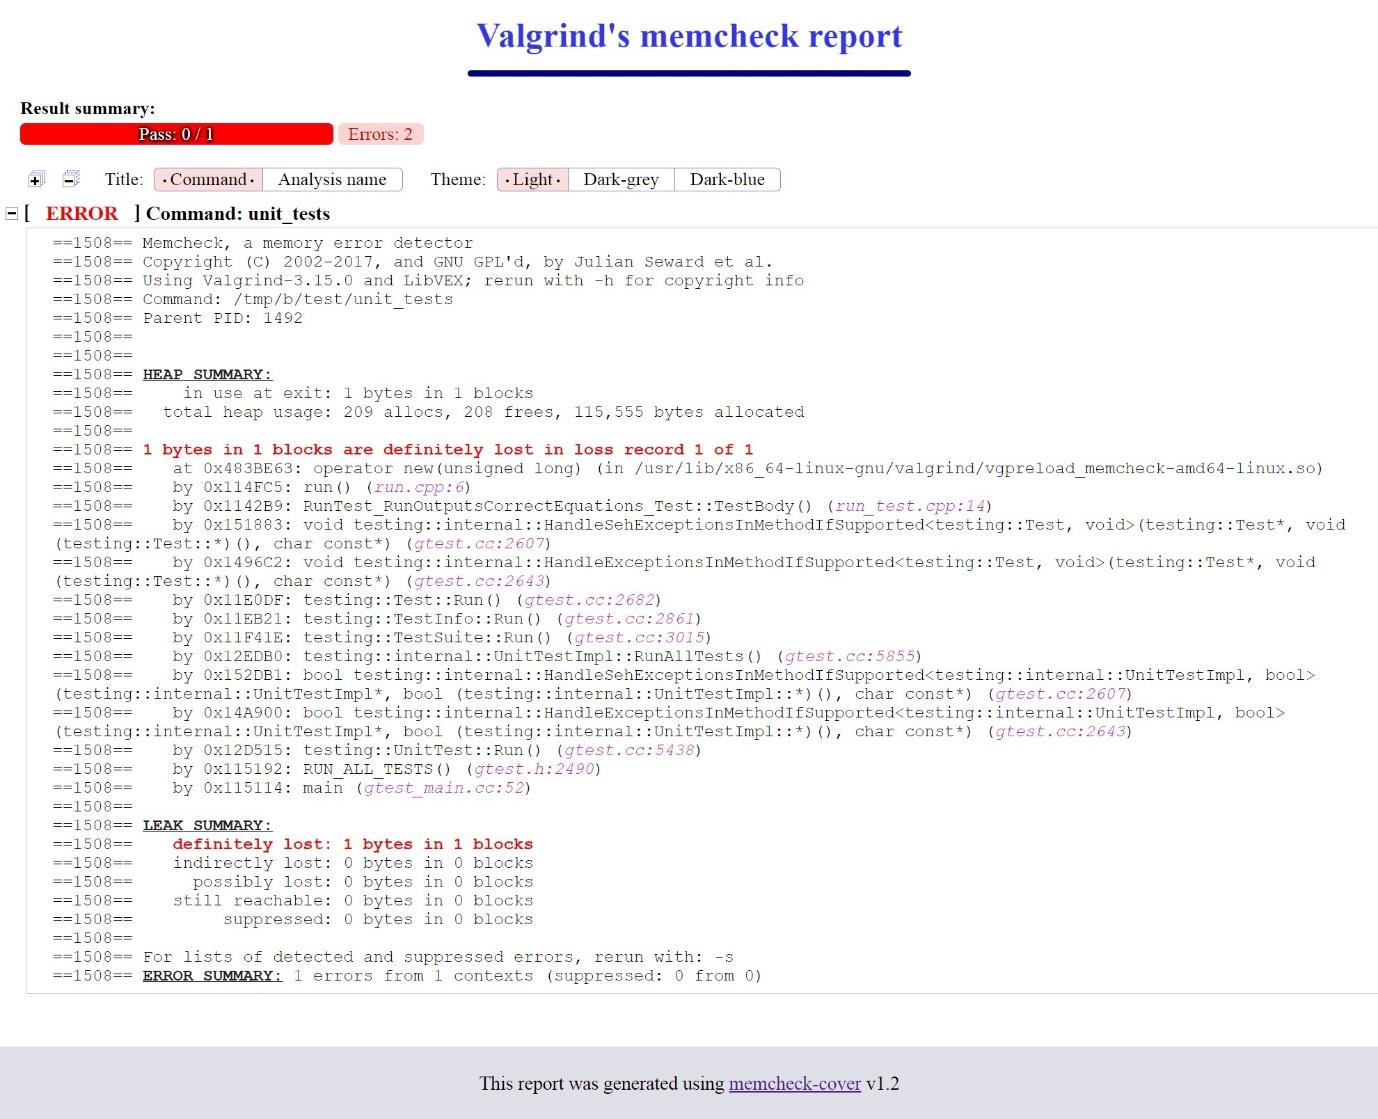
\includegraphics[width=0.8\textwidth]{content/3/chapter9/images/1.jpg}\\
Figure 9.1 – A report generated by memcheck-cover
\end{center}

This neat little project is available on GitHub (\url{https://github.com/Farigh/memcheck-cover}); it requires Valgrind and gawk (GNU AWK tool). To use it, we'll prepare a setup function in a separate CMake module. It will consist of two parts:

\begin{itemize}
\item 
Fetching and configuring the tool

\item 
Adding a custom target that executes Valgrind and generates a report
\end{itemize}

The configuration looks as follows:

\begin{lstlisting}[style=styleCMake]
# chapter09/04-memcheck/cmake/Memcheck.cmake

function(AddMemcheck target)
	include(FetchContent)
	FetchContent_Declare(
	memcheck-cover
		GIT_REPOSITORY https://github.com/Farigh/memcheckcover.git
		GIT_TAG release-1.2
	)
	FetchContent_MakeAvailable(memcheck-cover)
set(MEMCHECK_PATH ${memcheck-cover_SOURCE_DIR}/bin)
\end{lstlisting}

In the first part, we follow the same practices as with a regular dependency: include the FetchContent module, and specify the project's repository and desired Git tag with FetchContent\_Declare. Next, we initiate the fetch process and configure the path to the binary using the memcheck-cover\_SOURCE\_DIR variable set by FetchContent\_Populate (called implicitly by FetchContent\_MakeAvailable).

The second part of the function is creating the target to generate reports. We'll call it memcheck (so that it doesn't overlap with the previous valgrind target if we want to keep both options for some reason):

\begin{lstlisting}[style=styleCMake]
# chapter09/04-memcheck/cmake/Memcheck.cmake (continued)

	add_custom_target(memcheck
		COMMAND ${MEMCHECK_PATH}/memcheck_runner.sh -o
			"${CMAKE_BINARY_DIR}/valgrind/report"
			-- $<TARGET_FILE:${target}>
		COMMAND ${MEMCHECK_PATH}/generate_html_report.sh
			-i "${CMAKE_BINARY_DIR}/valgrind"
			-o "${CMAKE_BINARY_DIR}/valgrind"
		WORKING_DIRECTORY ${CMAKE_BINARY_DIR}
	)
endfunction()
\end{lstlisting}

This happens in two commands:

\begin{enumerate}
\item 
First, we'll run the memcheck\_runner.sh wrapper script, which will execute Valgrind's Memcheck and collect the output to the file provided with the -o argument.

\item 
Then, we'll parse the output and create the report with generate\_html\_report.sh. This script requires input and output directories provided with the -i and -o arguments.
\end{enumerate}

Both steps should be executed in the CMAKE\_BINARY\_DIR working directory so that the unit test binary can access files through relative paths if needed.

The last thing we need to add to our list files is, of course, a call to this function. It has the same pattern as AddValgrind:

\begin{lstlisting}[style=styleCMake]
# chapter09/04-memcheck/test/CMakeLists.txt (fragment)

include(Memcheck)
AddMemcheck(unit_tests)
\end{lstlisting}

After generating a buildsystem with the Debug config, we can build the target with the following:

\begin{tcblisting}{commandshell={}}
cmake --build <build-tree> -t memcheck
\end{tcblisting}

And then we can enjoy our formatted report. Well, to truly enjoy it we'll need to add that missing delete c; in run.cpp so that it stops complaining (or, better yet, use a smart pointer instead).








